\chapter{Derivation of relative dynamics equations} \label{chap:B}
The vector position from the centre of the Earth to the satellite 1 and the satellite 2 is given by
\begin{flalign}
\vec{p_1} &= R  \vec{\hat{x}} \\
\vec{p_2} &= R  \vec{\hat{x}} + x  \vec{\hat{x}} + y  \vec{\hat{y}}
\end{flalign}
the first time derivative and second time relative of $\vec{p_1}$ and $\vec{p_2}$ is computed:
\begin{flalign*}
\dot{\vec{p_1}} &= \dot{R}  \vec{\hat{x}} + R(\vec{w} \times \vec{\hat{x}}) 
\end{flalign*}
where $\vec{w}$ is the angular velocity vector and $\vec{w} = w  \vec{\hat{z}}$ due to the fact the position of the satellites stay all over the time in the plan $(\vec{\hat{x}},\vec{\hat{y}})$. Therefore, the first time derivative and the second time derivative are given by:
\begin{flalign*}
\dot{\vec{p_1}} &= \dot{R}  \vec{\hat{x}} + w R  \vec{\hat{y}} \\
\ddot{\vec{p_1}} &= \ddot{R}  \vec{\hat{x}} + w\dot{R}  \vec{\hat{y}} + \dot{w} R  \vec{\hat{y}} + w \dot{R}  \vec{\hat{y}} + wR  (\vec{w} \times \vec{\hat{y}}) \\
&= \ddot{R}  \vec{\hat{x}} + 2w\dot{R}  \vec{\hat{y}} - w^2R  \vec{\hat{x}} \\
\dot{\vec{p_2}} &= \dot{\vec{p_1}} +  \dot{x}  \vec{\hat{x}} + x w  \vec{\hat{y}} + \dot{y}  \vec{\hat{y}} - y w  \vec{\hat{x}} \\
&= \dot{\vec{p_1}} + (\dot{x} - yw)  \vec{\hat{x}} + (xw + \dot{y})  \vec{\hat{y}} \\
\ddot{\vec{p_2}} & = \ddot{\vec{p_1}} + (\ddot{x} - \dot{y}w - y\dot{w})  \vec{\hat{x}} + (\dot{x} - yw) w  \vec{\hat{y}} + (\dot{x}w + x\dot{w} + \ddot{y})  \vec{\hat{y}} - (xw + \dot{y}) w  \vec{\hat{x}} \\
&= \ddot{\vec{p_1}} + (\ddot{x} - 2\dot{y}w - y\dot{w} - xw^2)  \vec{\hat{x}} + (\ddot{y} + 2\dot{x}w + x\dot{w} - yw^2)  \vec{\hat{y}}
\end{flalign*}
Furthermore, The Newton law gives:
\begin{flalign}
	m\ddot{\vec{p_1}} &= \vec{F_{grav,1}} + \vec{F_{drag,1}} + \vec{F_{dist,1}}	\label{eq:l3} \\
	m\ddot{\vec{p_2}} &= \vec{F_{grav,2}} + \vec{F_{drag,2}} + \vec{F_{dist,2}} 	\label{eq:l4} \\
	\Rightarrow \ddot{\vec{p_2}} - \ddot{\vec{p_1}} &= \frac{1}{m}(\Delta \vec{F_{grav}} + \Delta \vec{F_{drag}} + \Delta \vec F_{dist}) 	\label{eq:l5}
\end{flalign}
with m is the mass of both satellites. The gravity is given by the universal law of gravitation:
\begin{flalign*}
\frac{\vec{F_{grav,1}}}{m} &= -G\frac{m_{earth}}{||\vec{R}||^3} \vec{R} \\
\frac{\vec{F_{grav,2}}}{m} &= -G\frac{m_{earth}}{||\vec{R} + \vec{r}||^3} (\vec{R} + \vec{r})
\end{flalign*}
where $\vec{r} = (x,y)$ is the vector from the satellite 1 to the satellite 2. The denominateur can be approximated using:
\begin{flalign*}
||\vec{R} + \vec{r}||^{-3} &= ||\vec{r}|| \\
%||\vec{R} + \vec{r}||^{-3} &= ||(\vec{R} + \vec{r})\cdot(\vec{R} + \vec{r})||^{\frac{-3}{2}} \\
%&= ||\vec{R} \cdot \vec{R} + \vec{r} \cdot \vec{r} + 2\vec{R} \cdot \vec{r}||^{\frac{-3}{2}} \\
%&= R^{-3}||1 + \frac{\vec{r} \cdot \vec{r}}{R^2} + 2\frac{\vec{r} \cdot \vec{R}}{R^2}||^{\frac{-3}{2}}
\end{flalign*}
%Due to the fact the $r << R$, the second term can be neglected and by using the approximation $(1 + x)^q = 1 + qx$ when $x << 1$. The expression can be approximated by:
%\begin{flalign*}
%||\vec{R} + \vec{r}||^{-3} &= R^{-3}(1 - 3\frac{\vec{r} \cdot \vec{R}}{R^2}) \\
%&= R^{-3}(1 - 3\frac{x}{R})
%\end{flalign*} 
and thus, the difference between the gravity force on satellite 2 and the the gravity force on 1 is:
\begin{flalign*}
\vec{F_{grav,2}} - \vec{F_{grav,1}} &\approx -\frac{\mu}{R^3}\vec{r} \\
%\vec{F_{grav,2}} - \vec{F_{grav,1}} &\approx -G \frac{m_{earth}}{R^3} ((1 - 3\frac{x}{R}) (\vec{R} + \vec{r}) - \vec{R}) \\
%&\approx -G \frac{m_{earth}}{R^3} (\vec{r} - 3x \cdot \vec{\hat{x}} + 3 \frac{x}{R} \vec{r}) \\
%&\approx -\frac{\mu}{R^3} (-2x \cdot \vec{\hat{x}} + y \cdot \vec{\hat{y}})
\end{flalign*} 
with $\mu = G  m_{earth}$, The drag force can be modelling be using \eqref{eq:teor}:
\begin{flalign*}
	\vec{F_{drag,1}} &= -u_1 ||\dot{\vec{p_1}}|| \dot{\vec{p_1}}\\
	& = -u_1 ||\dot{\vec{p_1}}|| (\dot{R}  \vec{\hat{x}} + wR  \vec{\hat{y}}) \\
	\vec{F_{drag,2}} &= -u_2 ||\dot{\vec{p_2}}|| \dot{\vec{p_2}} \\
	& = -u_2 ||\dot{\vec{p_2}}|| ((\dot{R} + \dot{x} - yw) \vec{\hat{x}} + (wR + xw + \dot{y})  \vec{\hat{y}})
\end{flalign*}
Therefore, the \eqref{eq:l3} becomes:
\begin{equation}
\left\{
	\begin{aligned}
		&\ddot{R} - w^2R = -\frac{\mu}{R^2} -\frac{u_1}{m} ||\dot{\vec{p_1}}|| \dot{R} + \frac{F_{dist,1,x}}{m} \\
		&2w\dot{R} + \dot{w}R = -\frac{u_1}{m} ||\dot{\vec{p_1}}|| wR + \frac{F_{dist,1,y}}{m}
	\end{aligned}
\right.
\end{equation}
and the \eqref{eq:l5} gives:
\begin{equation}
\left\{
	\begin{aligned}
		& \ddot{x} - 2\dot{y}w - y\dot{w} - xw^2 = -x\frac{\mu}{R^3} + \frac{u_1}{m} ||\dot{\vec{p_1}}|| \dot{R} - \frac{u_2}{m} ||\dot{\vec{p_2}}||(\dot{R} + \dot{x} - yw) + \frac{\Delta F_{dist,x}}{m}\\
		&\ddot{y} + 2\dot{x}w + x\dot{w} - yw^2 = -y\frac{\mu}{R^3} + \frac{u_1}{m}||\dot{\vec{p_1}}||wR - \frac{u_2}{m}||\dot{\vec{p_2}}||(wR + xw + \dot{y}) + \frac{\Delta F_{dist,y}}{m}
	\end{aligned}
\right.
\label{eq:l7}
\end{equation}
The operating point is the position ($x^{*},y^{*}$) of the satellite 2 in the frame of satellite. $x^{*}$ and $y^{*}$ can be computed from \figref{fig:operating_pt}.
\begin{figure}[H]
	\centering
	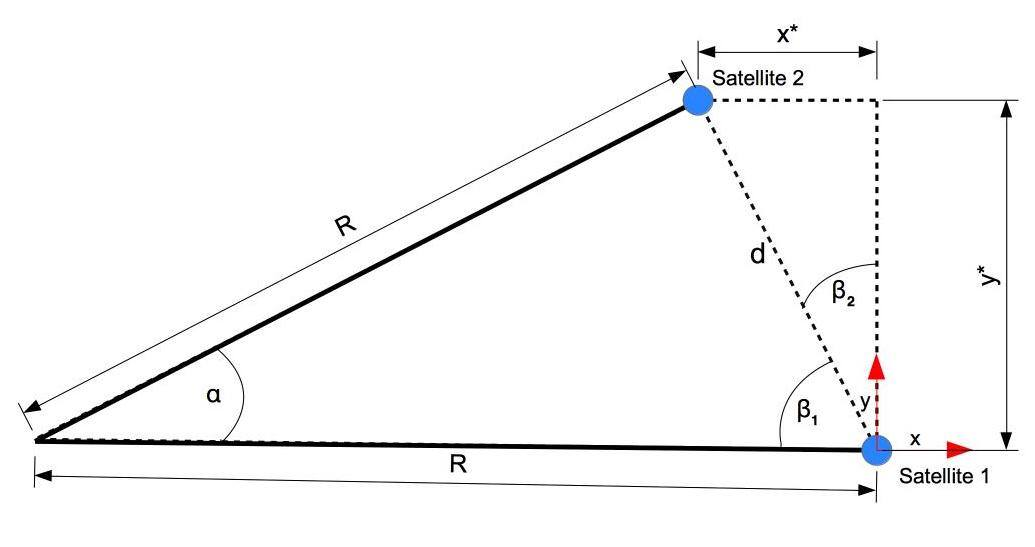
\includegraphics[width=0.75\linewidth]{figures/operating_point}
	\caption{Operating point}
	\label{fig:operating_pt}
\end{figure} 
Using trigonometry relations:
\begin{flalign*}
d &= 2Rsin(\frac{\alpha}{2}) \\
x^{*} &= -dsin(\beta_2) \\
&= -dsin(\frac{\alpha}{2}) \\
&= -2Rsin(\frac{\alpha}{2})^2 \\
y^{*}  &= dcos(\frac{\alpha}{2}) \\
&= 2Rsin(\frac{\alpha}{2})cos(\frac{\alpha}{2}) \\
&= Rsin(\alpha)
\end{flalign*}
with $\alpha$ is the desired angle between satellite and so $\beta_2 = 90^{\circ} - \beta_1 = 90^{\circ} - (90^{\circ} - \frac{\alpha}{2}) = \frac{\alpha}{2}$. Therefore we change the coordinate reference as following:
\begin{flalign*}
x &\Leftarrow x - x^{*}  \\
y &\Leftarrow y - y^{*}  
\end{flalign*}
Thus, the equations \eqref{eq:l7} become:
\begin{equation}
\left\{
\begin{aligned}
	& \ddot{x} - 2\dot{y}w - (y + y^{*})\dot{w} - (x + x^{*})w^2 = \\
	&-(x + x^{*})\frac{\mu}{R^3} + \frac{u_1}{m} ||\dot{\vec{p_1}}|| \dot{R} - \frac{u_2}{m} ||\dot{\vec{p_2}}||(\dot{R} + \dot{x} - (y + y^{*})w) + \frac{\Delta F_{dist,x}}{m}\\
	&\ddot{y} + 2\dot{x}w + (x + x^{*})\dot{w} - (y + y^{*})w^2 =\\
	& -(y + y^{*})\frac{\mu}{R^3} + \frac{u_1}{m}||\dot{\vec{p_1}}||wR - \frac{u_2}{m}||\dot{\vec{p_2}}||(wR + (x + x^{*})w + \dot{y}) + \frac{\Delta F_{dist,y}}{m}
\end{aligned}
\right.
	\label{eq:la1}
\end{equation}
\subsection{Linearisation of the relative dynamics eqations} \label{sec:C}
From the equations \eqref{eq:la1} and assuming that the radius is constant and the angular velocity equals to $w = \sqrt{\frac{\mu}{R^3}}$, a linearization of the system can be derived using some approximations. The state is defined as :
\begin{flalign*}
	s = [x \ \dot{x} \ y \ \dot{y}]^\mathsf{T}
\end{flalign*}
Moreover, the norm of the velocity of both satellite is assumed to be equal and to be constant ($||\vec{\dot{p_1}}|| = ||\vec{\dot{p_2}}|| = C$). Therefore, the nominal system is given by:
\begin{equation}
\left\{
\begin{aligned}
& \dot{s_1} = s_2 \\
& \dot{s_2} = 2ws_4 - u_2\frac{y^{*}wC}{m} \\
& \dot{s_3} = s_4 \\
& \dot{s_4} = -2ws_2 - (u_2 - u_1)\frac{wRC}{m}
\label{eq:statespaceassumption}  
\end{aligned}
\right.
\end{equation}
using the approximation $\dot{x}$, $y << y^{*}$ and $x, x^{*}$, $\frac{\dot{y}}{w} << R$. 